W matematyce, grafy można zdefiniować jako graficzną reprezentację danych,
w której wartości są przedstawione w pewien uporządkowany sposób, zwykle w relacji do siebie nawzajem.
„\textit{Stanowią wygodny aparat do modelowania różnych obiektów, (...) i odpowiednio interpretowane
- mogą zawierać pewne informacje}”\cite{Wloch2008}.

Teoria grafów to dziedzina matematyki zajmująca się badaniem właściwości grafów,
będąca bardzo ważnym narzędziem w wielu „\textit{dziedzinach od rachunku operacyjnego, chemii, po genetykę, lingiwistykę
oraz od elektroniki i geografii po socjologię i architekturę}”\cite{Wilson2012}.
Grafy dają możliwość zobrazowania pewnych modeli, co jest szczególnie korzystne w analizie wzorców.
W kontekście grafów warto podkreślić ich zastosowanie poza teoretycznymi analizami.

W dziedzinach informatycznych, grafy stanowią fundament wielu algorytmów, takich jak algorytmy przechodzenia,
algorytmy najkrótszej ścieżki, drzew rozpinających, czy modeli sieci.
Przykładem może być tutaj wyszukiwanie najkrótszej trasy, chociażby w nawigacji GPS,
gdzie węzły odpowiadają skrzyżowaniom, a krawędzie drogom.
W przypadku znajdowania najbardziej optymalnych tras, warto wymienić takie algorytmy jak A*, Bellmana-Forda czy Dijkstry.

\begin{figure}[ht]
	\centering
	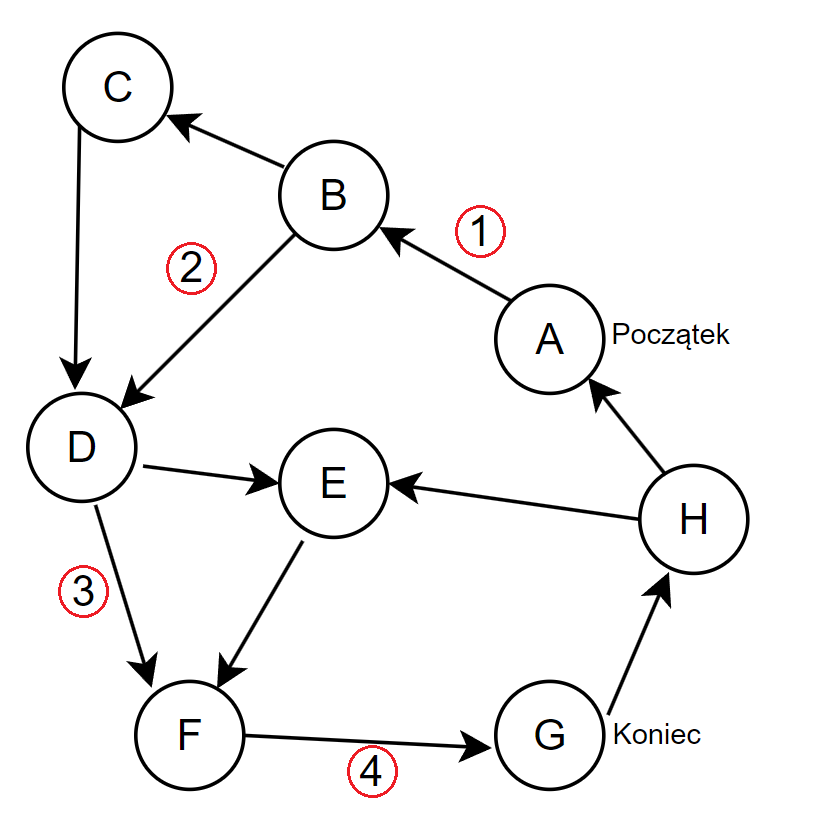
\includegraphics[height=6cm]{partials/images/intro_shortest_path.png}
	\caption{Przykład grafu z wyznaczoną najkrótszą ścieżką od węzła A do G}
    \label{Fig:intro-1}
\end{figure}

Duże znaczenie mają również w reprezentacji i modelowaniu struktur danych, takich jak bazy danych.
Najczęściej stosowane bazy danych, tj. relacyjne, zbudowane są w sposób, który grafy mogą doskonale zobrazować -
węzły będą kolumnami w tabelach a połączenia między nimi to krawędzie, reprezentujące relacje.

\begin{figure}[ht]
	\centering
	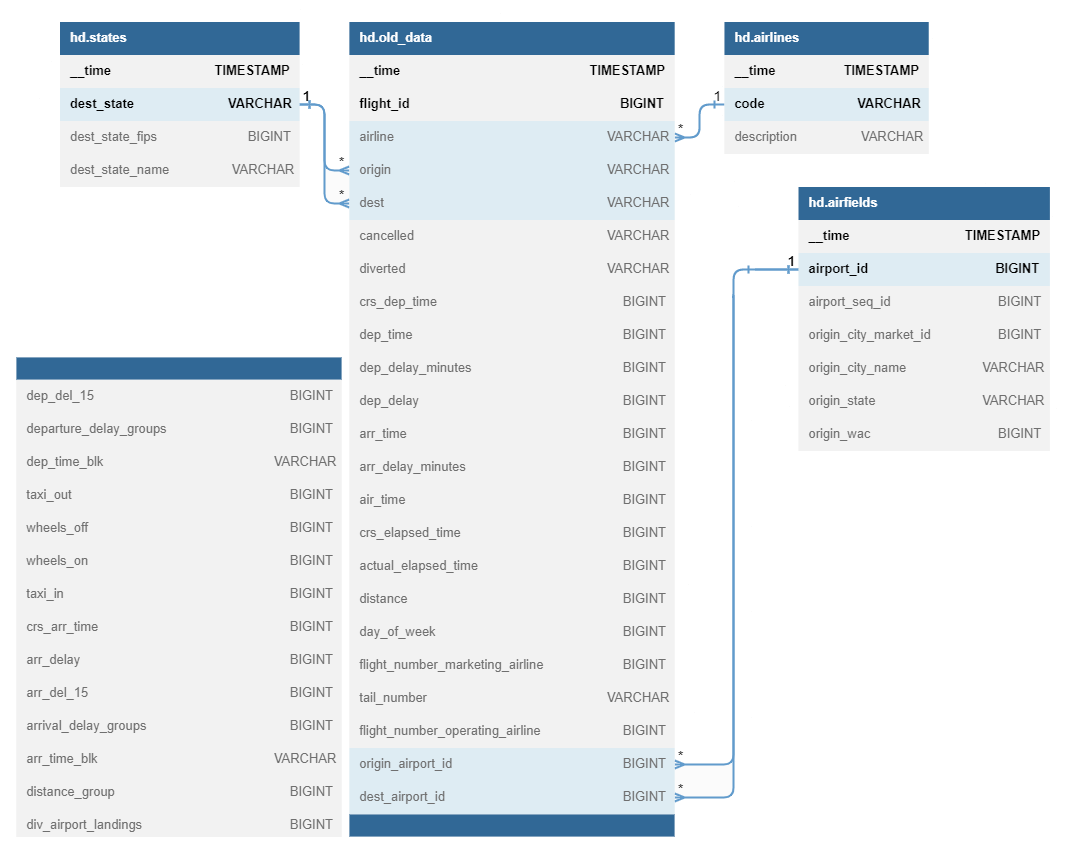
\includegraphics[height=7.5cm]{partials/images/intro_database.png}
	\caption{Przykładowy schemat relacyjnej bazy danych}
    \label{Fig:intro-2}
\end{figure}

W biologii, grafy pełnią ważną rolę w modelowaniu układu nerwowego, sieci białek,
szlaków metabolicznych oraz interakcji między genami.
W genetyce wykorzystuje się je między innymi do analizy drzew filogenetycznych,
co pozwala chociażby na śledzenie relacji ewolucyjnych między organizmami,
z liśćmi reprezentującymi żywe organizmy, a węzłami pośrednimi jako ich wspólnymi przodkami \cite{Erciyes2023}.

%////////TO-DO//////////%
Natomiast w chemii, grafy służą do reprezentacji struktury molekularnej związków chemicznych,
umożliwiając naukowcom analizę ich właściwości i reaktywności.

W dziedzinie lingwistyki, grafy wykorzystywne są w modelowaniu struktury języka.
Wykorzystywane są, na przykład, w analizie morfologicznej czy syntaktycznej.
Dzięki nim możliwe jest również lepsze zrozumienie i przetwarzanie języka naturalnego przez komputery,
co stanowi podstawę technologii takich jak tłumaczenie automatyczne czy rozpoznawanie mowy.

W dziedzinie uczenia maszynowego i sztucznej inteligencji, grafy odgrywają kluczową rolę w reprezentacji danych i wiedzy.
Grafy wiedzy, które łączą różne informacje, umożliwiają tworzenie zaawansowanych systemów rekomendacyjnych i chatbotów.
Wykorzystanie grafów w analizie danych pozwala odkrywać ukryte zależności i wzorce, co jest niezwykle cenne w dzisiejszej erze big data

Rozpoznawanie wzorców, nam ludziom, pozwala na szybszą naukę przez rozpoznawanie czegoś, co już wcześniej widzieliśmy.
W bardzo dużym uproszczeniu, algorytmy uczenia maszynowego działają w podobny sposób.
Gdy model zostanie prawidłowo nauczony na pewnych danych, jest w stanie rozpoznawać podobne wzorce w innych,
nigdy wcześniej nie widzianych miejscach.
Grafy znajdują także zastosowanie w analizie sieci społecznych, gdzie pomagają w badaniu relacji między ludźmi,
takich jak przyjaźnie, współpraca zawodowa czy wpływy.
Dzięki analizie grafów można lepiej zrozumieć dynamikę grup społecznych i przepływ informacji,
co jest szczególnie istotne w marketingu i polityce.

Podsumowując, grafy są niezwykle wszechstronnym narzędziem, które znajduje zastosowanie w wielu dziedzinach nauki i technologii.
Ich zdolność do reprezentowania skomplikowanych struktur i relacji w sposób zrozumiały i przystępny jest nieoceniona.
Dzięki grafom możliwe jest analizowanie i przetwarzanie informacji w bardziej efektywny sposób. 

Celem pracy jest zobrazowanie owej zależności, na przykładzie nauczenia sieci neuronowej,
w taki sposób, by po wytrenowaniu na kilku typach grafów stworzonych sztucznie,
model był w stanie rozpoznać dane wzorce i je nazwać, w przestrzeni rzeczywistej.